% !TEX root=../../mt-motion-analysis.tex
\chapter{Introduction} \label{ch:intro}
Among the physically active, young to middle aged population injuries to, e.g., knee or hip are common. In a study by Thorborg et al., 49\% of the questioned sub-elite football players in Denmark reported they had issues with hip and/or groin pain during the previous season \cite{Thorborg2017}. Among serious injuries, rupture of the \gls{acl} is one of the more severe and common and the incidence rate among athletes is about 1.5 per 10000 athlete-exposure. The injury rate for women is 1.7 times higher than it is for men \cite{Montalvo2019}. Treatment of such injuries is a debated subject and whether surgery yields better results is difficult to say \cite{Krause2018, Monk2016}. Independently of the treatment, the patient needs to undergo a rehabilitation process, potentially for as long as 2 years \cite{Nagelli2017}.
Apart from the rehabilitation, an injury may also lead to long term physical impairments, such as joint instability \cite{Ageberg2002} and increased risk of knee ostearthritis (OA) \cite{Lohmander2007}, as well as increased risk of depression \cite{Crichlow2006} and re-injury \cite{Paterno2012}.

% Moses et al. show annual \gls{acl} injury incidence rates of up to 1.62\% for amateur athletes \cite{Moses2012}

The \gls{acl}, seen in Figure \ref{fig:acl}, is one of the ligaments connecting the femur (thigh bone) with the tibia (shin bone) and is a key structure for providing stability in the knee \cite{Duthon2006}. Injuries to the \gls{acl} commonly occurs without any direct contact from e.g. other athletes. Instead a typical injury mechanism is a sudden change of direction or velocity while the knee bears weight \cite{Wetters2016}.

\begin{figure}
  \centering
  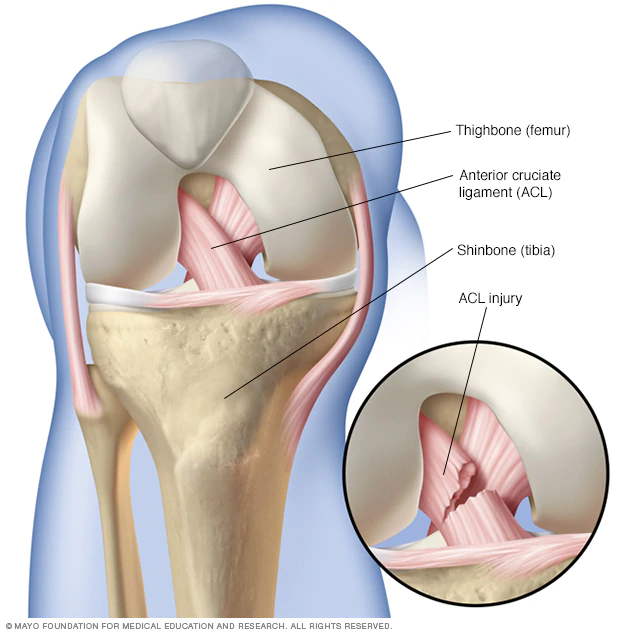
\includegraphics[width=0.6\textwidth]{files/figs/intro/acl.png}
  % \caption{Illustration of the position of the ACL in the knee and a ruptured ACL. Image from \cite{MayoACL}.}
  \caption{Illustration of the position of the ACL in the knee. Image from \cite{MayoACL}.}
  \label{fig:acl}
\end{figure}

% \section{ACL anatomy}

\section{Postural Orientation Errors}
The ability to uphold the alignment of body segments, both in relation to each other and the surroundings, is called postural orientation \cite{Horak2006}. Altered postural orientation, for example \glspl{poe}, has been seen to increase the risk of suffering new injuries \cite{Hewett2005}. Hence this is suggested to be an important measure during rehabilitation and before return to sports. 3D motion capture systems are considered to be the "gold standard" for measurement of postural orientation. This is, however, an expensive and time consuming procedure, requiring specific resource in terms of laboratories and experts to perform the measurements. A potential alternative, more suitable for clinical use, is visual assessments of 2D measurements (i.e., videos) \cite{Nae2020}.

There is not one established method for visual assessments of postural orientation, but Nae et al. presented a test battery where up to six segment specific \glspl{poe} were assessed for five different functional tasks. Each \gls{poe} was scored on an ordinal scale from 0 to 2 \cite{Nae2017, Nae2020b}.
A detailed explanation of the \gls{poe}-task combinations can be found in Appendix~\ref{app:poe-task}. This scoring system is the foundation of this thesis, but, in this work, we only study the deviation of trunk-, deviation of pelvis-, femoral valgus-, and \gls{kmfp} \glspl{poe} for the \gls{sls} task. The criteria for the assessments of the \glspl{poe} are presented in Table \ref{tab:poes} and the \gls{sls} task is described below. When a patient is assessed four-five repetitions are performed, each being scored according to Table \ref{tab:poes}. A total segment-specific score is then calculated as the median of these repetitions.

\subsubsection{Single-leg squat, SLS} \label{sec:SLS}
The subject performs a squat standing on one leg to a knee angle of approximately $60\degree$ before returning to extension. The exercise is repeated five times and the entire movement is used to assess the POEs \cite{Nae2020}. %An illustration is shown in Figure \ref{}.

\begin{table}
 \centering
 \caption{Descriptions for the visual assessment of segment specific POEs evaluated in this thesis. Table taken from \cite{Nae2020}.}
 \label{tab:poes}
 \footnotesize
 % {\renewcommand{\arraystretch}{1.2}
 {\tabulinesep=0.8mm
 \begin{tabu}[t]{c|ccc}

  % \hline
  % {\renewcommand{\arraystretch}{1}
  \multicolumn{1}{l}{\begin{tabular}[t]{@{}l@{}}\textbf{Segment-specific}\\\textbf{\glspl{poe}}\end{tabular}} &
  \multicolumn{1}{l}{\begin{tabular}[t]{@{}l@{}}\textbf{Scoring of 0:}\\\textbf{Good (no \gls{poe})}\end{tabular}} &
  \multicolumn{1}{l}{\begin{tabular}[t]{@{}l@{}}\textbf{Scoring of 1:}\\\textbf{Fair (minor \gls{poe})}\end{tabular}} &
  \multicolumn{1}{l}{\begin{tabular}[t]{@{}l@{}}\textbf{Scoring of 2:}\\\textbf{Poor (major \gls{poe})}\end{tabular}}\\ \hline \hline
  % {\renewcommand{\arraystretch}{1}
  \multicolumn{1}{l}{\begin{tabular}[t]{@{}l@{}}\textbf{Deviation}\\
                                                \textbf{of trunk}\\
                                                \textbf{in any plane}\end{tabular}} &
  \multicolumn{1}{l}{\begin{tabular}[t]{@{}l@{}}The absence of a trunk\\
                                                position into forward\\
                                                lean, lateral lean\\
                                                and/or rotation\\
                                                indicates no \gls{poe}\end{tabular}} &
  \multicolumn{1}{l}{\begin{tabular}[t]{@{}l@{}}A slight position of the\\
                                                trunk into forward lean,\\
                                                lateral lean and/or\\
                                                rotation indicates\\
                                                minor \gls{poe}\end{tabular}} &
  \multicolumn{1}{l}{\begin{tabular}[t]{@{}l@{}}A clear position of\\
                                                the trunk into forward\\
                                                lean, lateral lean\\
                                                and/or rotation\\
                                                indicates major \gls{poe}\end{tabular}} \\
  % {\renewcommand{\arraystretch}{1}
  \multicolumn{1}{l}{\begin{tabular}[t]{@{}l@{}}\textbf{Deviation}\\
                                                \textbf{of pelvis}\\
                                                \textbf{in any plane}\end{tabular}} &
  \multicolumn{1}{l}{\begin{tabular}[t]{@{}l@{}}The absence of\\
                                                pelvis into lateral\\
                                                deviation, pelvic tilt\\
                                                and/or rotation of\\
                                                pelvis respectively\\
                                                indicates no \gls{poe} \end{tabular}} &
  \multicolumn{1}{l}{\begin{tabular}[t]{@{}l@{}}A slight position of the\\
                                                pelvis into lateral\\
                                                deviation, pelvic tilt\\
                                                and/or rotation of\\
                                                pelvis respectively\\
                                                indicates minor \gls{poe} \end{tabular}} &
  \multicolumn{1}{l}{\begin{tabular}[t]{@{}l@{}}A clear position of the\\
                                                pelvis into lateral\\
                                                deviation, pelvic tilt\\
                                                and/or rotation of\\
                                                pelvis respectively\\
                                                indicates major \gls{poe} \end{tabular}} \\
  % {\renewcommand{\arraystretch}{1}
  \multicolumn{1}{l}{\begin{tabular}[t]{@{}l@{}}\textbf{Femoral}\\
                                                \textbf{valgus} \end{tabular}} &
  \multicolumn{1}{l}{\begin{tabular}[t]{@{}l@{}}The absence of\\
                                                femoral valgus\\
                                                indicates no \gls{poe} \end{tabular}} &
  \multicolumn{1}{l}{\begin{tabular}[t]{@{}l@{}}A slight position of\\
                                                femoral valgus\\
                                                indicates minor \gls{poe} \end{tabular}}&
  \multicolumn{1}{l}{\begin{tabular}[t]{@{}l@{}}A clear position of\\
                                                femoral valgus\\
                                                indicates major \gls{poe} \end{tabular}}\\
  % {\renewcommand{\arraystretch}{1}
  \multicolumn{1}{l}{\begin{tabular}[t]{@{}l@{}}\textbf{Knee}\\
                                                \textbf{Medial-to-Foot}\\
                                                \textbf{Position} \end{tabular}} &
  \multicolumn{1}{l}{\begin{tabular}[t]{@{}l@{}}Mid-point of patella\\
                                                is in line with or\\
                                                lateral to the\\
                                                second toe \end{tabular}} &
  \multicolumn{1}{l}{\begin{tabular}[t]{@{}l@{}}Mid-point of patella\\
                                                is placed medial to\\
                                                the second toe \end{tabular}} &
  \multicolumn{1}{l}{\begin{tabular}[t]{@{}l@{}}Mid-point of patella\\
                                                is clearly placed\\
                                                medial to the big toe \end{tabular}}
\end{tabu}}

\end{table}

Although visual assessments based on 2D videos are a time and resource efficient way of evaluating \glspl{poe} compared to 3D motion capture systems, it is still a time consuming method. Automating such assessments could hopefully improve the quality of the rehabilitation, both by allowing the physiotherapist to spend more time with the patient, but also by helping to direct the focus of the training to a specific segment in need of improvement. It could also give more accurate and less biased results compared to human assessments.

\section{Related work}
A study by the National Board of Health and Welfare in Sweden from 2019 show that the use of \gls{ai} systems in the Swedish healthcare is still fairly limited. At the date of the report such systems were used for 59 applications, of which 27 were based on some machine learning approach. The learning based methods were most commonly used for diagnosis and decision support, mainly based on different types of image analysis \cite{soc2019}. Within the research community the situation is different, here machine learning applied in a medical field is very widespread, for instance in medical imaging fields such as radiology and ultrasound, but also EKG, anamnesis, and mental health. The introduction of wearable devices and cheaper IoT devices are deemed to be important factors for the digitalization of healthcare \cite{Topol2019}.

Machine learning has also been used in the field of physiotherapy and rehabilitation. Kianifar et al. estimated joint poses from IMU data using extended Kalman filters. Based on these joint positions they classified the quality of \gls{sls} movements using Support Vector Machines, Linear Multinomial Logistic Regression, and Decision Trees \cite{Kianifar2016}. Liao et al. used combinations of Gaussian Mixture Models and \glspl{dnn} to calculate quality scores for movements during rehabilitation based on 3D joint positions captured with a Microsoft Kinect \cite{Liao2020}.

% https://ieeexplore.ieee.org/document/7592162 lol
% https://pubmed.ncbi.nlm.nih.gov/29204327/ lololol
% https://www.sciencedirect.com/science/article/pii/S2468781218301590?via%3Dihub

\section{Focus of this work}
This work should be seen as a proof of concept showing that these kinds of assessments can be automated, allowing physiotherapists to help patients in a more efficient way. Due to limitations in time and labeled data only four \glspl{poe} for the \gls{sls} task was evaluated. After some initial studies it was decided to use 2D body joint positions, i.e., 3D reconstruction from the videos was not evaluated.

% SKRIV LITE MER H'R HOPPAS LAG, TYP OM JAG KOMMER P[ NGT VID RESULTAT ELLER NGT...

\section{Thesis organization}
After this first chapter, where the background and rationale for this thesis has been presented, some deep learning background is introduced in Chapter \ref{ch:dl}. Chapters \ref{ch:hpe} and \ref{ch:tsc} present methods for estimating human body joints and classifying time series, both important for this work. The methods developed as part of this thesis is provided in Chapter \ref{ch:method}. Finally, the results are presented and discussed in Chapter \ref{ch:results}. Chapter \ref{ch:conclusions} summarizes the work and suggests improvements for the future.

% \section{avgr'nsningar eller typ m]l med detta arbete}
% typ om att bara SLS analyseras? och lite s[nt.. kanske att 3d inte utv'rderas? eller att det utv'rderades litgrann??
%
%
% skriv om risker med bias fr dataset osv... kansek ska n'mnas i dl-kapitlet?
